
\begin{figure}[H]
    \centering
    % FROM: TODO
    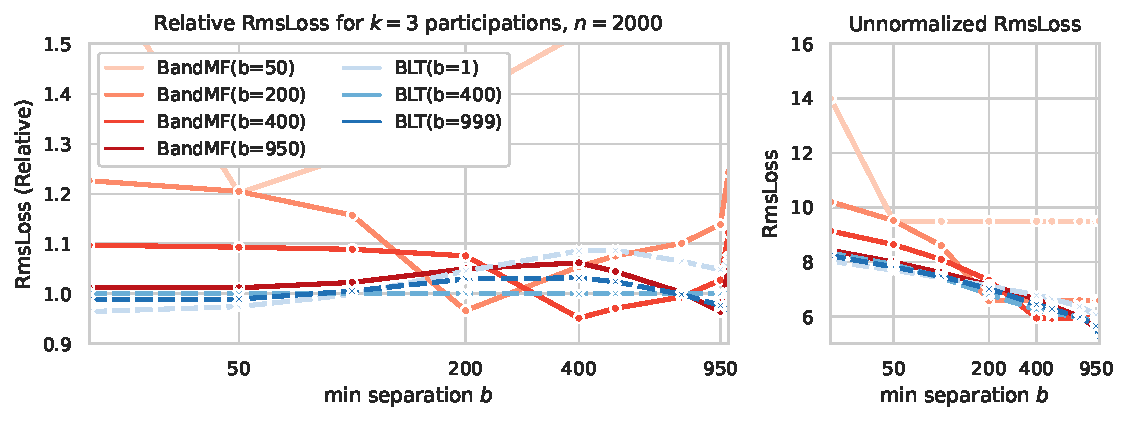
\includegraphics[width=\linewidth]{images/rmse_vary_min_sep_k3.pdf}
    \caption{Comparison of \bandmf and \blts with $\nd = 2000$ and $k=3$ participations, varying the min-separation $\minsep$. The \blts were optimized for \rmsloss. The $x$-axis is shown on a log-scale. The left panel gives loss relative to the $\bltm(b=400)$ mechanism, while the right panel gives the same data on an unnormalized $y$-axis scale.}
    \label{fig:rmse_k3}
\end{figure}

\begin{figure}[H]
    \centering
    % FROM: TODO
    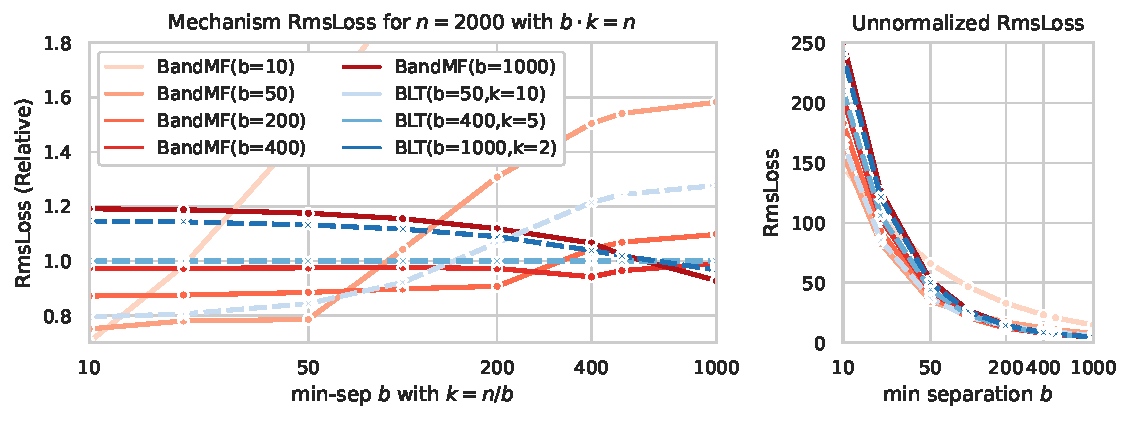
\includegraphics[width=\linewidth]{images/rmse_nkb.pdf}
    \caption{Comparison of \bandmf and \blts with $\nd = 2000$, varying $\minsep$ such that $\maxpart = \nd / \minsep$ is an integer. The \blts were optimized for \rmsloss. The $x$-axis is shown on a log-scale. The left panel gives loss relative to the $\bltm(b=400)$ mechanism, while the right panel gives the same data on an unnormalized $y$-axis scale.}
    \label{fig:rmse_nkb}
\end{figure}


\paragraph{Robustness to Min-sep $b$} \cref{fig:rmse_k3} compares BLT to the strong baseline \bandmf, fixing $\nd = 2000$ and $k=3$ participations and varying the min-separation $\minsep$. We make three primary observations: 
\begin{enumerate*}[label=\color{purple}(\arabic*)]
\item 
%The optimization of the \bandmf mechanisms does not depend on $\maxpart$, and so implicitly is designed for the case where $\maxpart \sim \nd / \minsep$ and $b \geq \hat b$; 
The optimization of the \bandmf mechanisms implicitly assumes $b \sim \hat b$, and
as expected, near this regime \bandmf in fact (slightly) outperforms the \blts. 
\item However, when $b \ll \nd / \maxpart$,  the \blts perform better. 
\item Interestingly, \bandmf performs significantly worse than the \blts at $b=999$. In this case, the only participation patterns that actually have 3 participations are e.g. $\{0, 999, 1998\}$, $\{0, 1000, 1999\}$ --- importantly, only the columns $\{0, 1, 999, 1000, 1998, 1999\}$ can ever occur in a 3-participation pattern. Because the columns of $\bfC$ for \bandmf all have the same column norm, this fact cannot be exploited. However, because of their Toeplitz structure, columns 1998 and 1999 have smaller norms than other columns, and that is beneficial in this situation. 
\end{enumerate*}

The setting where $\maxpart$ is fixed and we vary $\minsep$ includes situations that should generally be avoided in practice. For example, if we had $\maxpart=3$, $\minsep=10$, and $\nd=2000$, this indicates we had enough data we should have been able to achieve $\minsep = \nd/\maxpart \approx 667$, and so $\minsep=10$ indicates a highly suboptimal data ordering.  Similarly, if we had $\maxpart=3$, $\minsep=999$, and $\nd=2000$, then we would have been better off stopping at $n=1998$, which would have ensured only $\maxpart=2$ participations and significantly decreased sensitivity (at presumably a small cost in learning performance compared to training for $\nd=2000$ iterations).

\cref{fig:rmse_nkb} shows the contrasting scenario (indicating an essentially optimal data ordering, general not possible in federated learning) that occurs when we fix $\nd = 2000$, and choose $\minsep$ that exactly divide $\nd$ so that we can take $\maxpart = \nd / \minsep$ exactly. \cref{fig:rmse_nkb} considers the worst-case max participation $k$ for given min-sep $b$ and total rounds $n$, and achieves generally larger \rmsloss. When $b \leq \hat b$, \bandmf slightly outperforms \blts, but \bandmf degrade more rapidly for $b \leq \hat b$. In general, the curves of \blts are more smoother across different min-sep $b$ in both \cref{fig:rmse_k3} and \cref{fig:rmse_nkb}.

\paragraph{Robustness to Total Rounds $n$} \cref{fig:rmse_vary_n} considers varying the number of steps of the mechanism actually executed for mechanisms optimzied for different $\nd$. \bandmf mechanisms can only be used up to the $\nd$ they are optimized for, but \blts naturally extend to any $\nd$. This figure demonstrates that again \blts are not particularly sensitive to the $\nd$ for which they are optimized. For this figure, the maximum number of participations is chosen to be the largest allowed given $\nd$ and $\minsep=400$ (i.e., $k=n/d$), leading to the stairstep behavior of the unnormalized \rmsloss in \cref{fig:rmse_vary_n} (Right). \bandmf optimizing for large $n$ performs well when the actual number of iterations executed is small, but optimizing for large $n$ encounters nontrivial as discussed in \cref{tab:mechanism_summary} and \cref{fig:faster}. Finally, these results show that only $\nbuf=2$ buffers is sufficient for good performance, or a $200\times$ memory savings compared to \bandmf with $\minsep=400$ bands.

%\zx{We potentially want another figure to compare with \tafull, and fix a $k$ when optimizing BLTs.}

\begin{figure}[htb]
    \centering
    % FROM: TODO
    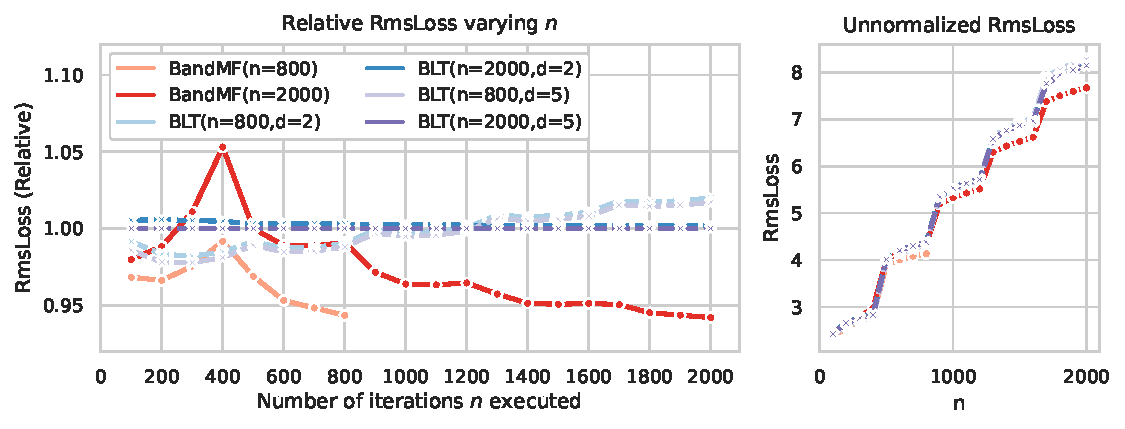
\includegraphics[width=\linewidth]{images/rmse_vary_n.pdf}
    \caption{Comparison of \bandmf and \blts optimized for $\nd=800$ and $\nd=2000$, and evaluated for $\nd$ up to the optimization target (for $\bandmf$) and over $[0, 2000]$ for the \blts. All mechanisms were optimized for min-separation (bands) $\minsep=400$. \blts with $\nbuf=2$ and $\nbuf=5$ perform almost equivalently; $\nbuf=1$ (not shown),is not sufficient with relative \rmsloss $> 1.07$.}
    \label{fig:rmse_vary_n}
\end{figure}

\begin{figure}[htb]
    \centering
    % FROM: https://colab.corp.google.com/drive/1_BRrt0jUniaOixKwasKDr7jiSToRwJLj#scrollTo=cYshzSOPA4wL&uniqifier=1
    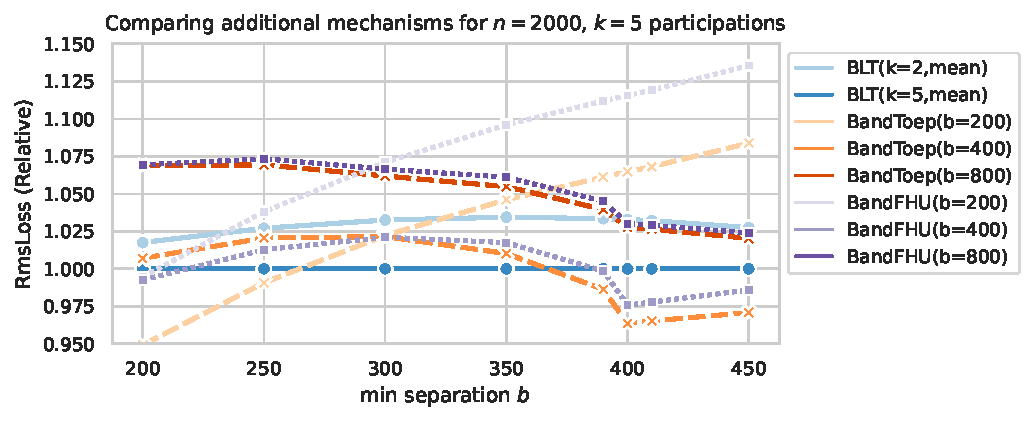
\includegraphics[width=\linewidth]{images/rmsloss_other_mechs.pdf}
    \caption{Comparison of mechanisms for $\nd=2000$ and $\maxpart=5$ participations, optimized for min-separation $\minsep = 400$ and compared for different actual values of min-separation. The setting is comparable to that of \cref{fig:rmse}, so only relative lines are given. 
    }
    \label{fig:other_mechs}
\end{figure}



\paragraph{Comparing \blt to \bandtoep and \bandfhu} Finally, we compare BLT-DP-FTRL to several other more recent mechanisms:
\begin{itemize}
    \item \bandtoep~\citep{mckenna2024scaling}, which optimizes banded Toeplitz matrices $\bfC$ for \bparticipation under \rmsloss. The primary advantage of this mechanism compared to \bandmf is that \bandtoep matrices can be optimized for much larger $\nd$. However, the runtime is the same as \bandmf, and the optimization is still slower than the optimization of \blts.
    \item \bandfhu~\citep{kalinin2024banded}, which uses prefixes of the optimal-for-single-participation \maxloss coefficients of \citet{fichtenberger2022constant} to form banded Toeplitz matrices. These will likely be worse than \bandtoep (which is specifically optimized for multiple participations), but require no mechanism optimization.
\end{itemize}
\cref{fig:other_mechs} shows that \blts are comparable or better to both of these approaches.